%% ------------------------------------------------------------------------- %%
\chapter{Fundamentação Teórica}
\label{cap:fundamentacao-teorica}

O problema de remoção de ruído telúrico em sinais astronômicos é de natureza interdisciplinar, o que implica na necessidade de compreender tanto a teoria da astronomia sobre espectros estelares, quanto a representação computacional do problema.
Neste capítulo são descritos conceitos básicos em espectroscopia astronômica, principalmente estelar, e algoritmos de processamento de sinais digitais utilizados na pesquisa, que em conjunto caracterizam o problema da contaminação telúrica de espectros estelares.

\section{Espectroscopia Astronômica} \label{astronomic-spectroscopy}

A espectroscopia é a técnica de dividir a luz, ou mais precisamente, a radiação eletromagnética, proveniente de um objeto em seus comprimentos de onda constituintes, o que resulta na formação de um espectro. Quando aplicada na astronomia, tem como objeto de estudo o espectro de radiação eletromagnética de diversos corpos celestes, como estrelas, planetas, nebulosas, galáxias e núcleos galácticos ativos.

Diferentes tipos de objetos celestes produzem diferentes tipos de espectro:  contínuo, de absorção e de emissão. Um espectro contínuo é um vetor de todos os comprimentos de ondas do espectro eletromagnético, arranjado de forma contínua. Ele é gerado pela observação de um corpo opaco quente, que seria o equivalente a observar diretamente o núcleo de uma estrela sem intervenção de matéria. Um espectro de absorção, ou espectro de linhas escuras, é gerado por um gás transparente frio em frente ao corpo opaco quente e está associado à absorção dos fótons da radiação em determinados comprimentos de onda. E por último, o espectro de emissão, ou espectro de linhas brilhantes, é gerado por um gás transparente que foi excitado por uma fonte de energia próxima, o que resulta na emissão de fótons de comprimentos de onda específicos. 

\begin{figure}[htb]
\centering
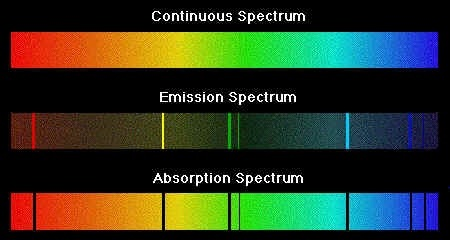
\includegraphics[width=10cm]{figuras/spectypes.jpg}
\caption{Os três tipos de espectro}
\label{fig:spectrum-types}
\end{figure}

Um objeto astronômico que é muito estudado pelos seus espectros são as estrelas. Por serem objetos quentes, rodeados de gases mais frios, estrelas emitem um espectro contínuo com linhas de absorção em comprimentos de onda característicos.

No final do século XIX, astrônomos perceberam que a análise cuidadosa do espectro de uma estrela fornece uma riqueza de detalhes sobre ela, incluindo sua temperatura efetiva, velocidade de rotação, velocidade de translação, densidade, composição química e metalicidade. Com a observação rotineira de espectros estelares em grandes números, estes pesquisadores notaram que era possível agrupar as estrelas baseado em suas características espectrais e assim surgiram diversos sistemas de classificação estelar. 

O sistema moderno de classificação de estrelas foi adotado em 1910 e foi criado por um time do observatório da Universidade de Harvard. Este sistema baseia-se nas intensidades relativas das linhas de absorção presentes no espectro. As variações nas linhas espectrais para diferentes estrelas são devidas principalmente à diferença de temperatura das camadas externas de gás na estrela, logo o sistema de classificação espectral é baseado na temperatura efetiva da estrela. 

As classes espectrais do sistema, em ordem decrescente de temperatura efetiva da estrela são: O, B, A, F, G, K, M. Cada uma dessas classes se subdivide em 10 (com os números de 0 a 9), sendo 0 a mais quente dentro da classe e 9 a mais fria.

\begin{figure}[htb]
\centering
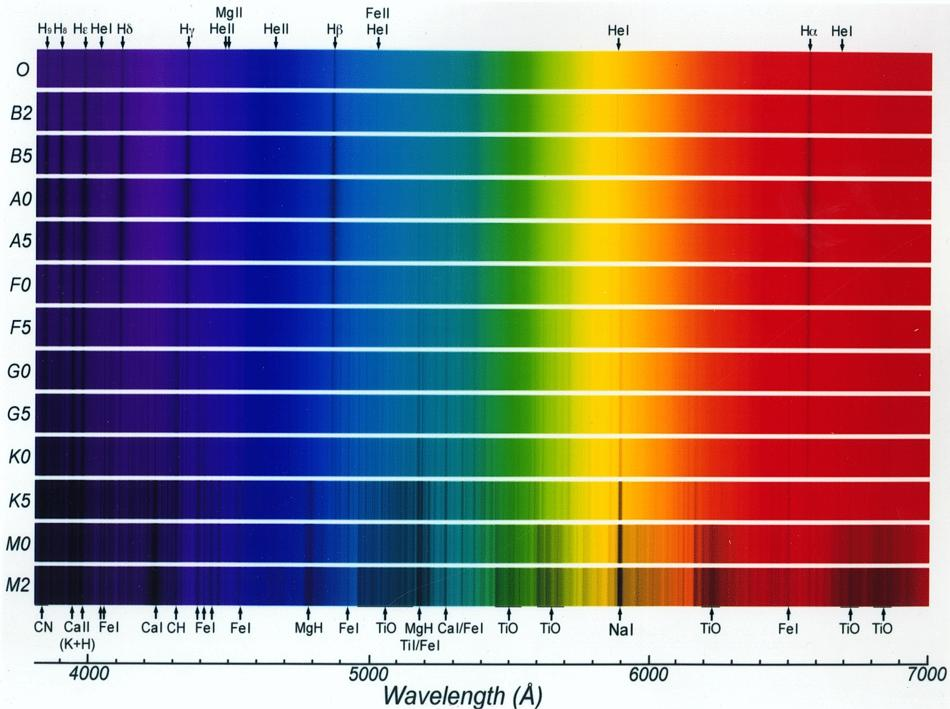
\includegraphics[width=10cm]{figuras/Spectra_Briley.jpg}
\caption{Tipos de espectro estelar}
\label{fig:stellar-spectrum-types}
\end{figure}

Na figura \ref{fig:stellar-spectrum-types}, é possível observar como diferentes linhas de absorção e bandas moleculares variam em força conforme a temperatura efetiva, ou tipo espectral, da estrela muda.

Os tipos espectrais das estrelas continuam sendo uma parte essencial para a pesquisa em astronomia, seja para auxiliar na descoberta de exoplanetas ou na interpretação da história da evolução das galáxias. 

\section{Sinal espectral}

No cerne do que é estudado pela espectroscopia astronômica está o sinal espectral. Para capturar o espectro de uma estrela é necessário utilizar um espectrógrafo, um instrumento presente em muitos telescópios que divide a radiação eletromagnética de um objeto celeste em seus respectivos comprimentos de onda.

Estes instrumentos de observação muitas vezes estão munidos de um CCD ou \textit{charge-coupled device}, um sensor eletrônico constituído por vários quadrados fotossensíveis, que representam os pixels de uma imagem. As imagens resultantes de uma observação do CCD passam por um processo de redução de dados, que envolve a transformação das imagens brutas em dados científicos utilizáveis.   

No caso dos espectros estelares, a redução de dados implica na extração de um espectro unidimensional à partir de uma imagem de CCD da estrela osbervada, também chamada de estrela de ciência. A figura \ref{fig:x0319-obs-spectrum} ilustra o espectro de uma estrela do \textit{X-Shooter Spectral Library} \citep{Chen2014TheXS}, uma coleção de estrelas observada pelo espectrógrafo de resolução média \textit{X-Shooter}, parte do \textit{Very Large Telescope array} (VLT), localizado no Cerro Paranal, Chile.  

\begin{figure}[htb]
\centering
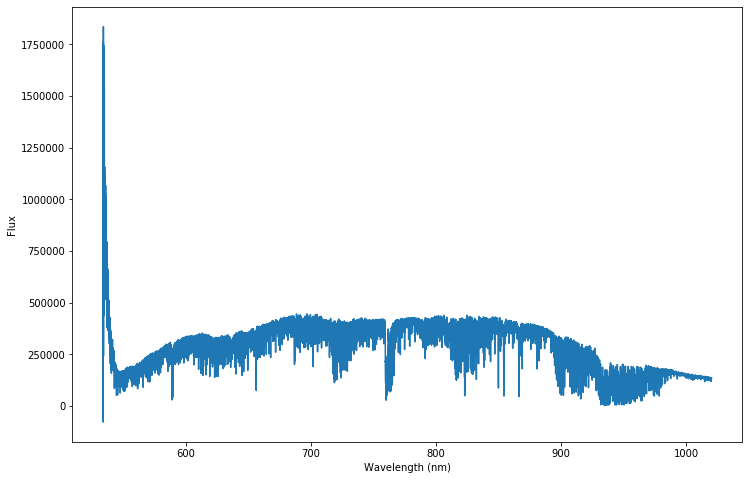
\includegraphics[width=15cm]{figuras/X0319_obs_spectrum.png}
\caption{O espectro observado da estrela X0319}
\label{fig:x0319-obs-spectrum}
\end{figure}

O espectro resultante da redução de dados é unidimensional no domínio do comprimento de onda da estrela e tem sua intensidade representada pelo fluxo, que é adimensional. O fluxo de um espectro estelar é geralmente reescalonado para o intervalo $[0, 1]$, de modo a padronizar a intensidade dos espectros. 

É possível observar que a figura \ref{fig:x0319-obs-spectrum} tem o formato esperado de um espectro estelar mencionado na seção \ref{astronomic-spectroscopy}: um espectro contínuo com a presença de várias linhas de absorção.


\section{Contaminação Telúrica}

Como as estrelas do \textit{X-Shooter Spectral Library}, a maioria das observações astronômicas são feitas em telescópios terrestres, ou seja, a partir do solo. Nesse caso, nem toda luz irradiada por um objeto celestre consegue ser capturada pelo espectrógrafo. Isto acontece pois, ao atravessar a atmosfera terrestre o sinal astronômico interage com moléculas como vapor de água e oxigênio, o que resulta na formação de novas linhas no espectro observado. Estas linhas são chamadas de linhas telúricas.

As linhas telúricas, quando misturadas no espectro original, contribuem para a criação de uma observação distorcida ou contaminada. A menos que seja corrigida, esta contaminação pode produzir erros e introduzir ruídos que reduzem a precisão dos dados observados, e consequentemente, dificultam o avanço de diversas pesquisas astronômicas.

Existem alguns procedimentos típicos usados hoje em dia para remover as linhas telúricas de um espectro de ciência. Um método popular consiste em aplicar uma divisão simples entre o espectro da observação e uma referência telúrica. Esta referência telúrica pode ser obtida de duas maneiras: através de um catálogo de estrelas padrão ou pela simulação de um espectro atmosférico teórico.

As estrelas padrão são estrelas quentes em rotação rápida de tipo espectral B ou A. Elas são escolhidas pois seus espectros não possuem características marcantes além de fortes linhas de hidrogênio. Para que o espectro de uma estrela padrão seja usado como uma referência telúrica, é necessário observá-la próxima em tempo, posição no céu e condições atmosféricas do espectro de ciência. Contudo, existem várias limitações fundamentais no nível de correção que pode ser obtido com o método da estrela padrão. Primeiramente, características estelares ainda podem estar presentes no espectro da estrela padrão, evidenciando que ela não é um modelo preciso da transmissão radiativa da atmosfera. Além disso, o tempo e a direção de observação das duas estrelas nunca será exatamente o mesmo, o que significa que a assinatura atmosférica de ambos os espectros também será diferente.

Devido às limitações das estrelas padrão, foi criado um método mais sofisticado e automatizado para obter uma referência telúrica: softwares de simulação do espectro atmosférico. Estes softwares utilizam modelos de transmissão radiativa da atmosfera para criar um espectro telúrico sintético, cujas condições de simulação são muito próximas às condições de observação da estrela de ciência. O modelo de transmissão atmosférica mais utilizado hoje em dia é o \textit{Line-By-Line Radiative Transfer Model (LBLRTM)} \citep{2005JQSRT..91..233C}, que fornece cálculos de radiância espectral com precisão e eficiência. Este modelo utiliza o HITRAN \citep{rothman2009hitran}, um acrônimo para \textit{High-resolution Transmission molecular absorption database}, uma base de dados de linhas e parâmetros espectroscópicos. 

Um exemplo desses softwares é o Molecfit \citep{smette2015molecfit}, uma ferramenta para a modelagem de linhas telúricas desenvolvido por astrônomos do \textit{European Southern Observatory}. De acordo com seus criadores, o Molecfit recupera o perfil atmosférico mais compatível com o tempo da observação da estrela de ciência. Isto envolve a utilização de um modelo de transmissão radiativa da atmosfera com uma base de dados espectral para recuperar atributos como a variação na temperatura, pressão e umidade em função da altitude da observação. É importante ressaltar que mesmo métodos como o Molecfit possuem suas limitações e podem, em certos casos, performar pior do que o método da estrela padrão.

Independente de como é gerado o referencial telúrico, a divisão simples do espectro observado por este indica que a ação da atmosfera na estrela é de natureza linear e multiplicativa. Em termos matemáticos, consideramos os espectros de ciência, telúrico e estelar sem contaminação como vetores $o$ (observado), $a$ (atmosfera) e $s$ (estrela), tal que:

\begin{equation*}
    o := \{o_1, o_2, \cdots, o_{n-1}\} \qquad a := \{a_1, a_2, \cdots, a_{n-1}\} \qquad s := \{s_1, s_2, \cdots, s_{n-1}\} 
\end{equation*}

os vetores possuem o mesmo comprimento e representam valores discretos do fluxo estelar ou atmosférico em intervalos igualmente espaçados de comprimento de onda. A contaminação telúrica do espectro de ciência nesta representação é a multiplicação dos elementos do vetor telúrico pelo estelar:

\begin{equation*}
    o = a \circ s
\end{equation*}

onde $\circ$ representa o produto de Hadamard, ou o produto par a par dos elementos do vetor. Esta representação tem como objetivo relaxar as restrições físicas do problema, de forma que seja possível aplicar algoritmos nos sinais que dependem da suposição de linearidade da contaminação telúrica.


\begin{itemize}
    \item filtros e pré-processamento de sinais (dúvidas se isso deve entrar aqui e se sim o que?)
\end{itemize}


\section{Alinhamento de sinais}

O estudo de sinais digitais, ou mais precisamente, a análise de séries temporais tem como objetivo estudar dados de séries temporais a fim de extrair estatísticas e características significativas dos dados. Um dos objetivos compreendidos pela análise de séries temporais é a mensuração da similaridade entre duas sequências. Este estudo se mostra necessário em diversas aplicações, principalmente em reconhecimento de fala produzidas por fontes sonoras, para saber se uma frase corresponde à outra, tanto em conteúdo quanto em velocidade.

Para se calcular a similaridade entre duas séries temporais pode ser usada a distância euclideana em pares de pontos de cada série que correspondem ao mesmo instante no domínio do tempo. Esta métrica funcionaria em sinais perfeitamente sincronizados no domínio do tempo e que se movem na mesma velocidade. No caso das sequências estarem dessincronizadas, pontos similares em cada uma delas começam a se afastar uns dos outros e a conclusão equivocada nesse caso é de que os sinais são pouco similares devido ao aumento da distância euclideana.

Um algoritmo mais roubusto que é utilizado para determinar a similaridade entre duas séries temporais chama \textit{Dynamic Time Warping (DTW)}. Este algoritmo acha uma correspondência ótima entre duas séries temporais, ou quaisquer dados que podem ser representados como sequências lineares, mesmo que estejam dessincronizados. Isto é feito com o deslocamento elástico das sequências para medir a similaridade de trechos com diferentes fases \citep{shou2005fast}. A figura \ref{fig:euclidean-vs-dtw-matching} ilustra como a DTW encontra uma correspondência mais intuitiva entre duas sequências, juntando regiões com formatos similares.

\begin{figure}[htb]
\centering
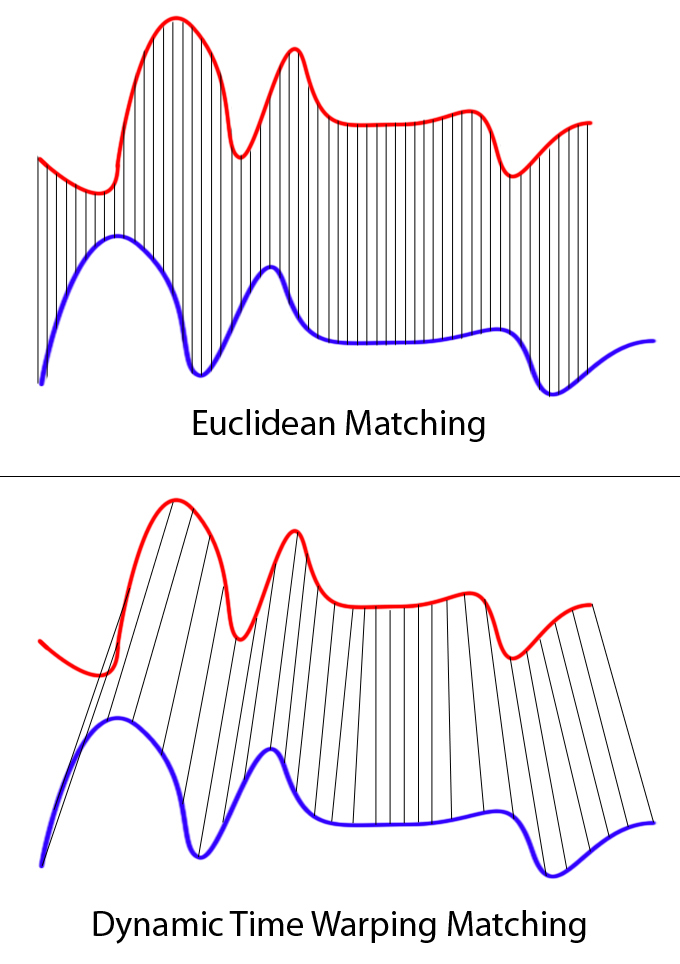
\includegraphics[width=7cm]{figuras/Euclidean_vs_DTW.jpg}
\caption{Diferença entre a correspondência euclideana e da DTW}
\label{fig:euclidean-vs-dtw-matching}
\end{figure}

explicar como funciona a dtw: matriz, programação dinamica, complexidade assintotica quadratica e metodos para acelerar algoritmo.


pq é necessario encontrar similaridade entre dois sinais, em que areas isso é usado, como é relevante nesse caso (falar dos microshifts e como eles dificultam a divisão dos sinais).

\begin{itemize}
    \item objetivo do alinhamento (pq surgiu a questão do alinhamento) 
    \item dtw
    \item fastdtw e restrições no caminho da matriz
\end{itemize}


